\documentclass{article}

\title{CS3101-P2-Databases}
\date{01/12/2017}
\author{150008859}

\setlength{\parskip}{1em}
\setlength{\parindent}{0em}

\usepackage{listings}
\usepackage{amsmath,amssymb,amsthm}
\usepackage{mathtools}
\usepackage{graphicx}
\usepackage{fancyvrb}
\usepackage{tikz}

\usepackage[section]{placeins}

\begin{document}

\newcommand{\udash}[1]{%
    \tikz[baseline=(todotted.base)]{
        \node[inner sep=1pt,outer sep=0pt] (todotted) {#1};
        \draw[dashed] (todotted.south west) -- (todotted.south east);
    }%
}%

\lstset {
  frameround=fttt
  ,language=SQL
  ,breaklines=true
  ,columns=flexible
}


\maketitle
\newpage

\section{Introduction}

This practical involved writing a front end in html, css and php for an audiobook streaming website.

\subsection{Features}

\subsubsection{Basic}

\begin{enumerate}
\item View all audiobooks 
\item View all audiobooks by author
\item View all reviews for audiobooks
\item Search for popular audiobooks
\item Purchase audiobook
\end{enumerate}

\subsubsection{Extensions}
\begin{enumerate}
\item Register/Login system
\item View all purchased books
\item Leave review on purchased audiobooks
\end{enumerate}

Screenshots are present at the end of this document (and in the report's image directory). 

\section{Design}

\subsection{Usage}

You may access the live version at:

\begin{lstlisting}
  https://saaz.host.cs.st-andrews.ac.uk/cs3301/
\end{lstlisting}

You may register an account using the register page and then login using a (made up) \textbf{email} and a \textbf{password}. (An already existing account is \textbf{test1@mail.com}:\textbf{12345}).

In the navigation bar, click Browse to view all books. Click Popular to view the most popular books. Click on My Books to view your purchase history.

Clicking a book's title take's you to that book's page.

Clicking the name of an author take's you to a list of books by that author.

A book's page contains an option to purchase a book, view all the reviews and the option to leave a review.

\subsection{Layout}

All classes can be found in the includes directory. I used the autoload technique to automatically include the class on instantiation \cite{php-autoload}.

All files that the user may interact are found in the top most parent directory.

I have used a style of PHP where in general each php file displays a feature or provides a service through some form of a request.

Some classes are able to fetch their own information from the database, for example the Book class.

\subsection{Usage of SQL}

I used the MySQL Improved interface in the OOP style \cite{php-mysqli}. This style involves using an object as opposed to passing handles to functions.

I used prepared statements. By reading the documentation, I found that prepared statements provide many advantages. In particular, the greatest advantage is the prevention of sql injection. Input is sent seperately after the query has been parsed, so the input does not interfere with the query. 

\subsection{Usage of HTML/CSS}

This is my first project in which I have used html/css. Hence, I adapted examples on w3schools. In particular, I adapted the examples for tables \cite{w3-schools-tables} and the navigation bar \cite{w3-schools-navigation}.

The tables are used for displaying the results of SQL queries in a neat way. The navigation bar allows user friendly navigation.

\subsection{Login and Registration System}

First, I added a new column to the person table for storing passwords.

Passwords are hashed using the bcrypt algorithm.

If an attacker had read access to the database, they wouldn't be able to obtain the cleartext version of the users password easily. 

I used bcrypt in particular because it automatically includes a salt, this means an attacker wouldn't be able to glean users with the same password or use precomputed rainbow tables.

In addition, bcrypt is easily configurable to increase the time taken to hash an input exponentially. This is better than using an algorithm like md5 which is computable very quickly. An attacker would have to expend significant computing power to calculate a hash.

During the login process, the password is verified using the recommended procedure in the documentation which involves using the password\_verify method.

Finally, the session variable is updated to store the user's id. The session variable is used to refer when purchasing, or leaving a review.

Logging out involves unsetting the user id stored in the session variable.

\subsection{Purchasing}

A ``Buy Now!'' link is displayed to the user when clicking on a book's title. This performs a request to purchase.php.

The purchase.php acts as a service. Given an isbn as a GET request, it will perform the purchase operation for a logged in user. The user can't accidently purchase it twice as a book can't be purchased if it has already been purchased.

After a book is purchased, the user is informed that they may listen to a book (although such a feature exists).

\subsection{Review}

A review is similar to a purchase. A form is submitted which performs a POST request on review.php.

Some extra care was taken to sanitize user input.

A malicious user may attempt to store code in a review so that it will executed when a review is fetched in an attack known as cross site scripting \cite{owasp-xss}.

Hence, the strip\_tags function is sanitize user input before it is stored into the database.

\section{Conclusion}

In conclusion, I found it enjoyable to create this audiobook streaming website.

In particular, it was interesting to research some of the security precautions taken into consideration when dealing with user input. A malicious user may try to inject sql queries, or attempt to execute malicious javascript in a client sided cross site scripting attack. In addition, storing passwords must be done very carefully just in case a malicious reader gets read access to the database to limit the impact on users.

The word count is 836.

\begin{thebibliography}{10}
  
\bibitem{php-autoload} 
  PHP autoload
  \\\texttt{http://php.net/manual/en/language.oop5.autoload.php}
  
\bibitem{php-mysqli}
  PHP MySQL Improved
  \\\texttt{http://php.net/manual/en/book.mysqli.php}

\bibitem{w3-schools-tables}
  w3schools html tables
  \\\texttt{https://www.w3schools.com/html/html\_tables.asp}

\bibitem{w3-schools-navigation}
  w3schools navigation bar
  \\\texttt{https://www.w3schools.com/css/css\_navbar.asp}

\bibitem{php-passwords}
  php hashing passwords
  \\\texttt{http://php.net/manual/en/faq.passwords.php}

\bibitem{owasp-xss}
  Owasp XSS attack
  \\\texttt{https://www.owasp.org/index.php/Cross-site\_Scripting\_(XSS)}


\end{thebibliography}


\section{Screenshots}

\begin{figure}[!htb]
  \caption{Login Page}
  \center
  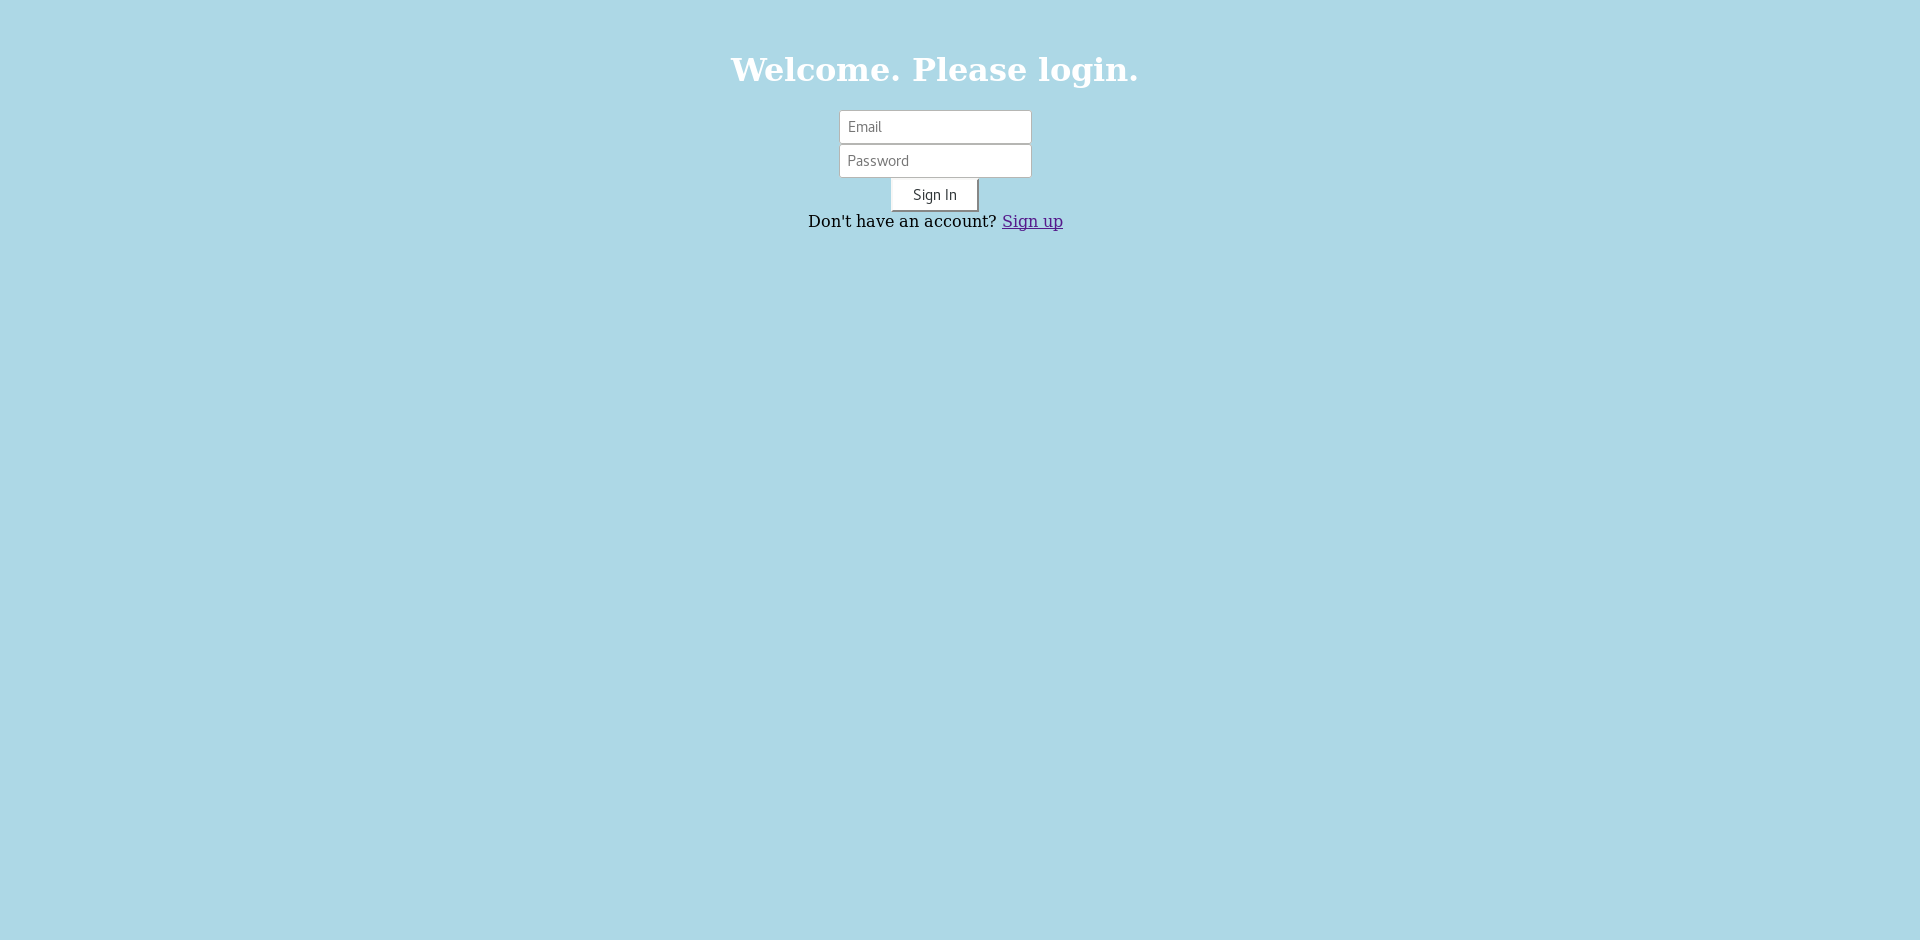
\includegraphics[scale=0.19]{image/login.png}
\end{figure}

\begin{figure}[!htb]
  \caption{Sign Up Page}
  \center
  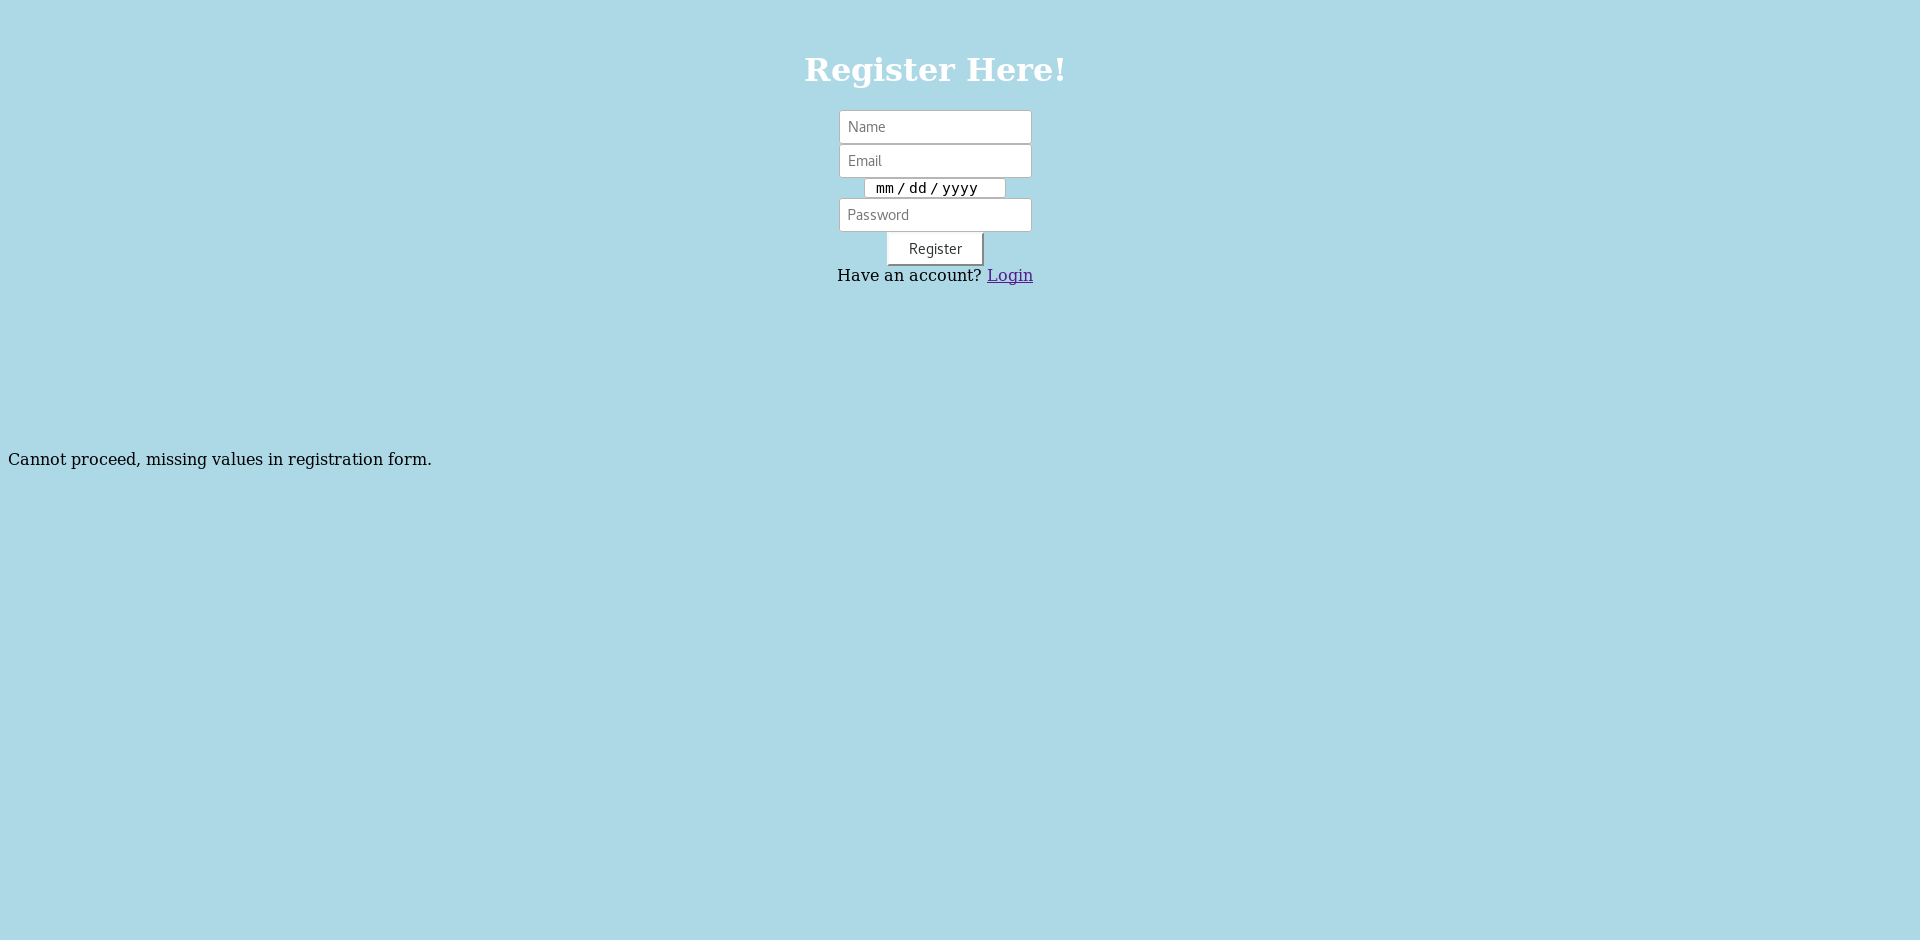
\includegraphics[scale=0.19]{image/register.png}
\end{figure}

\begin{figure}[!htb]
  \caption{Show all books}
  \center
  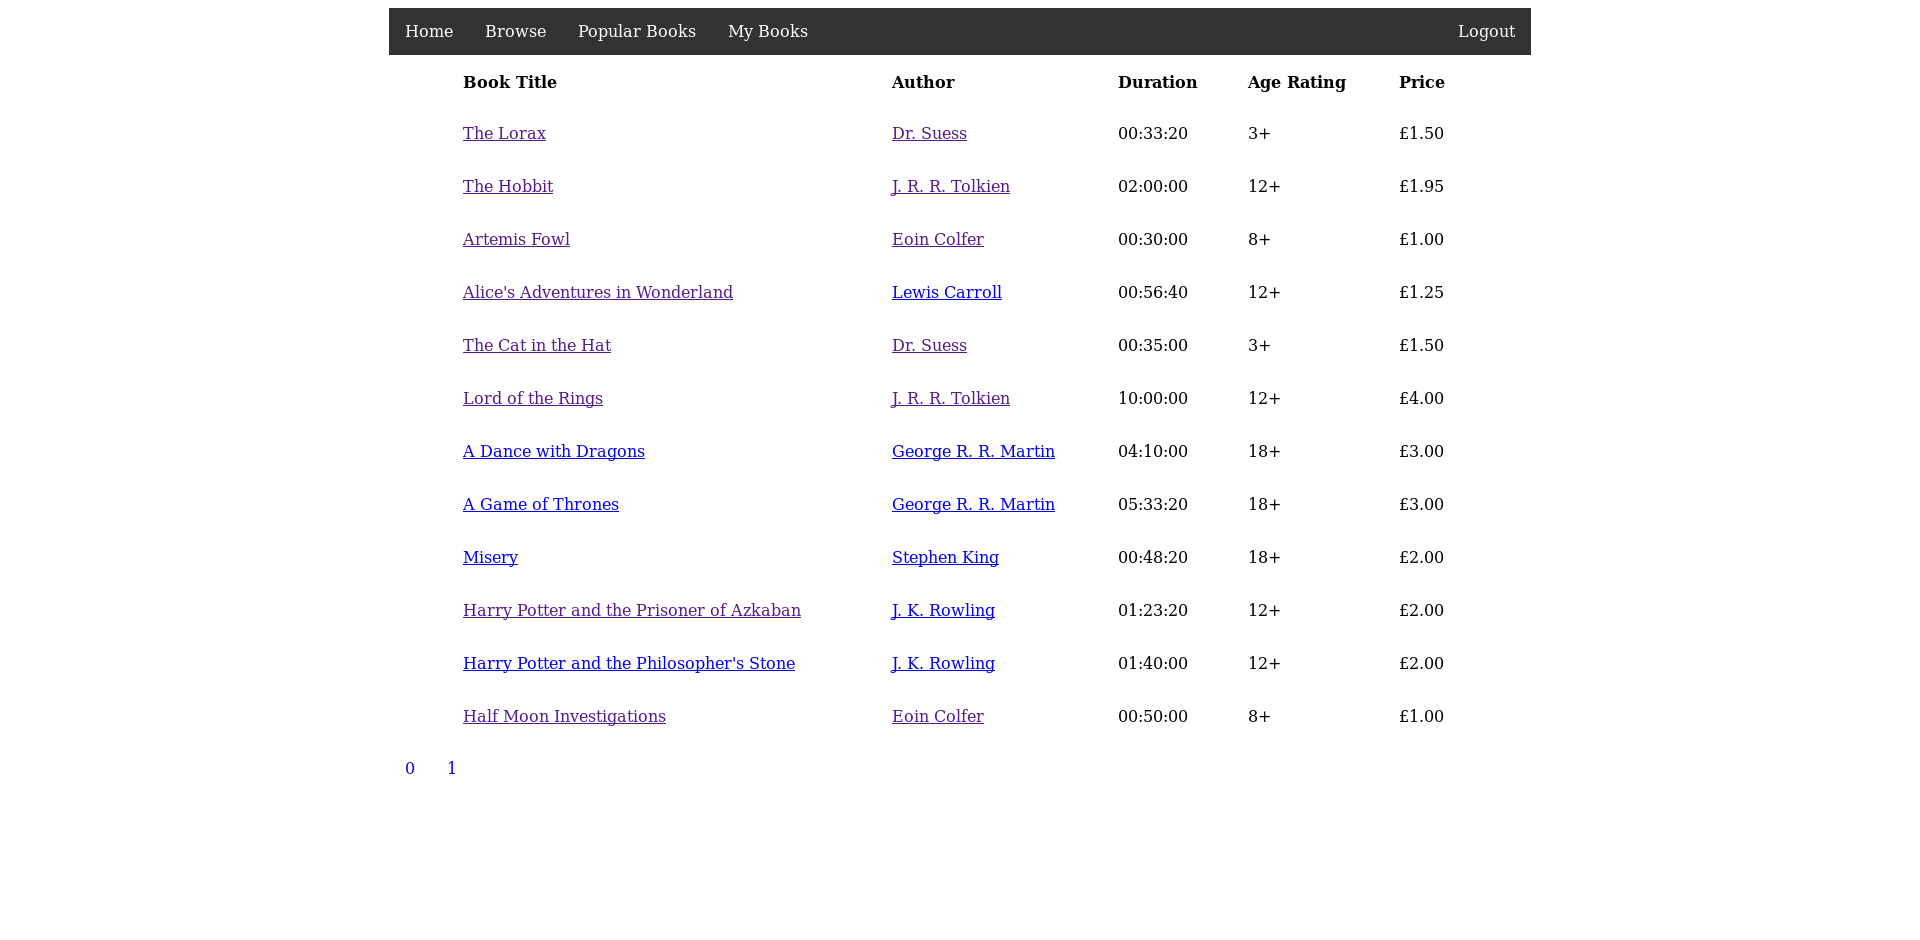
\includegraphics[scale=0.19]{image/browse.png}
\end{figure}

\begin{figure}[!htb]
  \caption{Popular Books}
  \center
  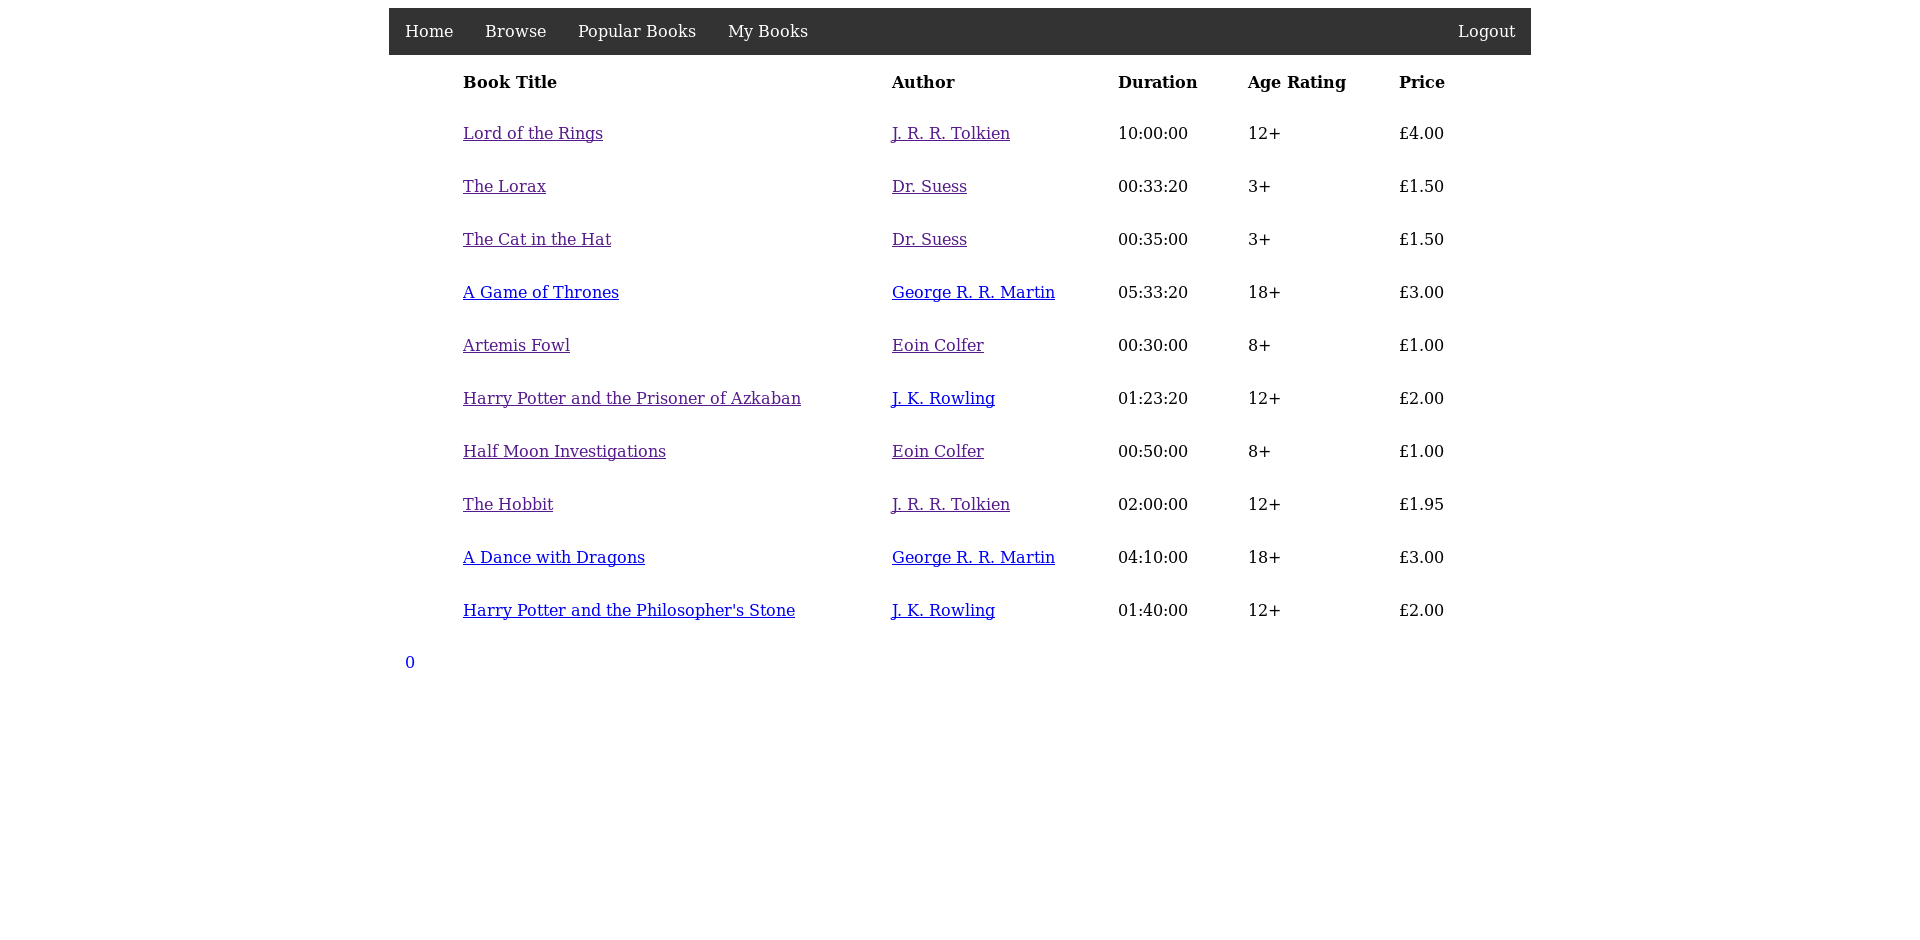
\includegraphics[scale=0.19]{image/popular.png}
\end{figure}

\begin{figure}[!htb]
  \caption{Book's by Dr Suess}
  \center
  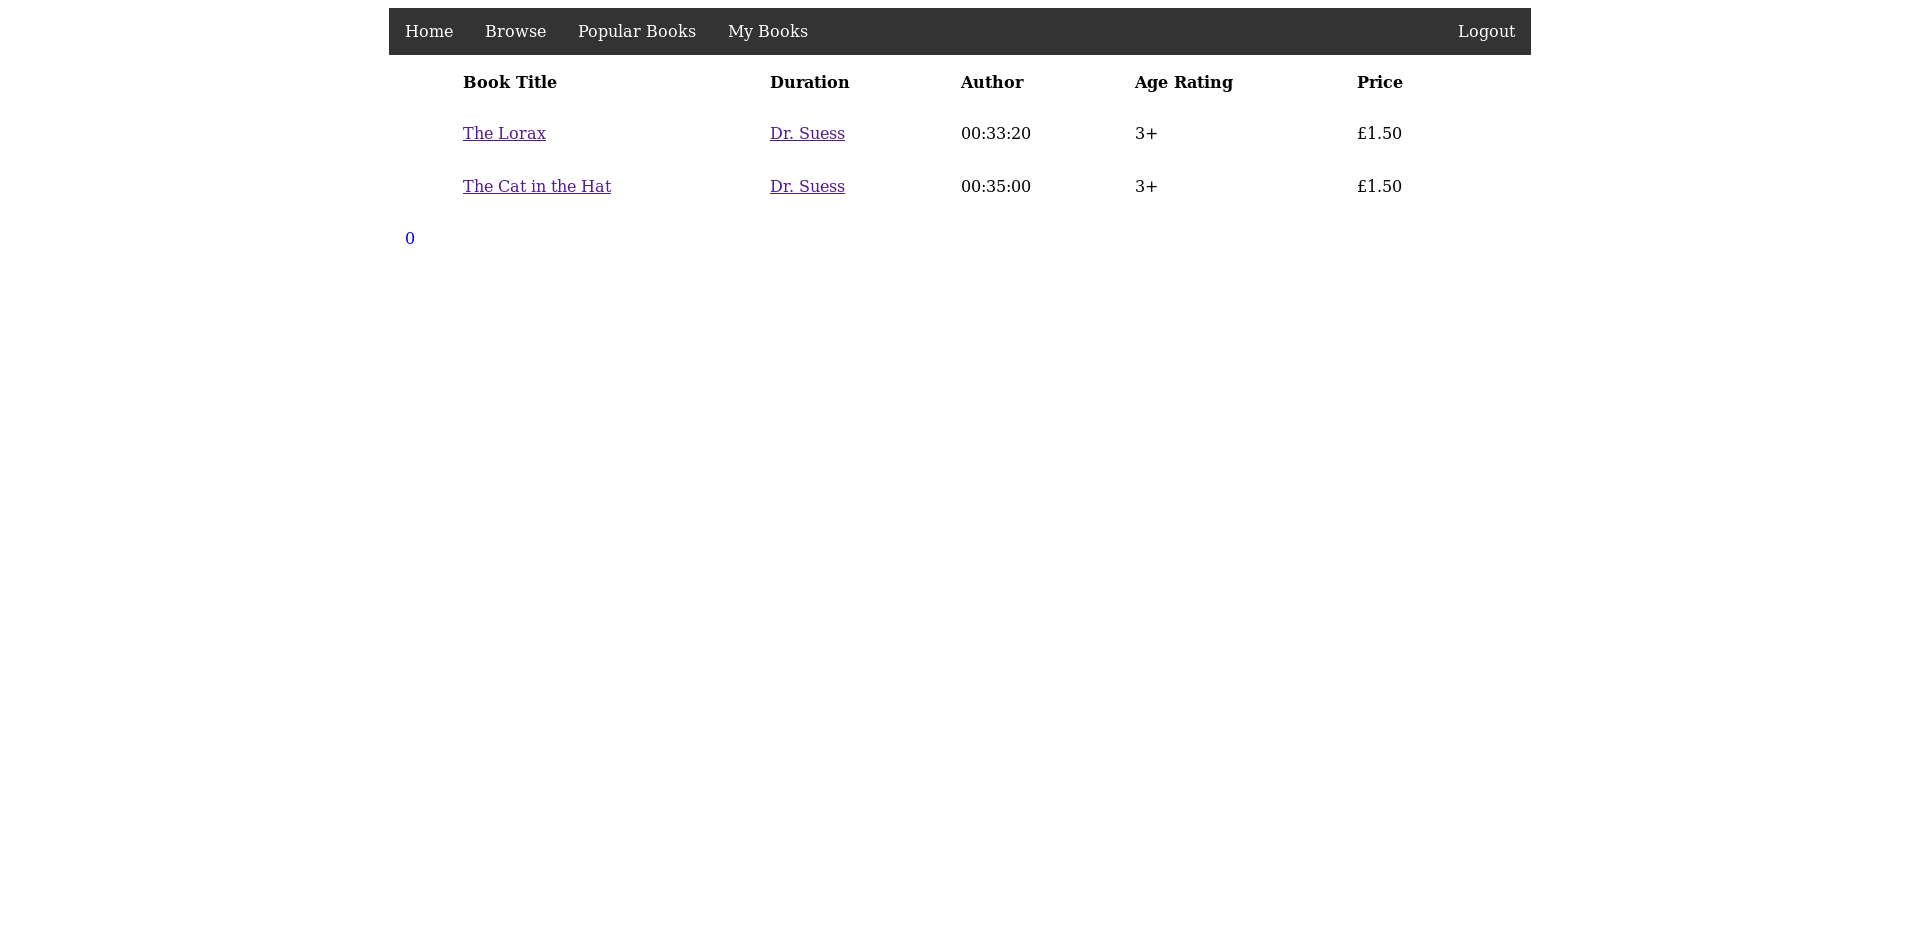
\includegraphics[scale=0.19]{image/author.png}
\end{figure}

\begin{figure}[!htb]
  \caption{The book page for The Lorax}
  \center
  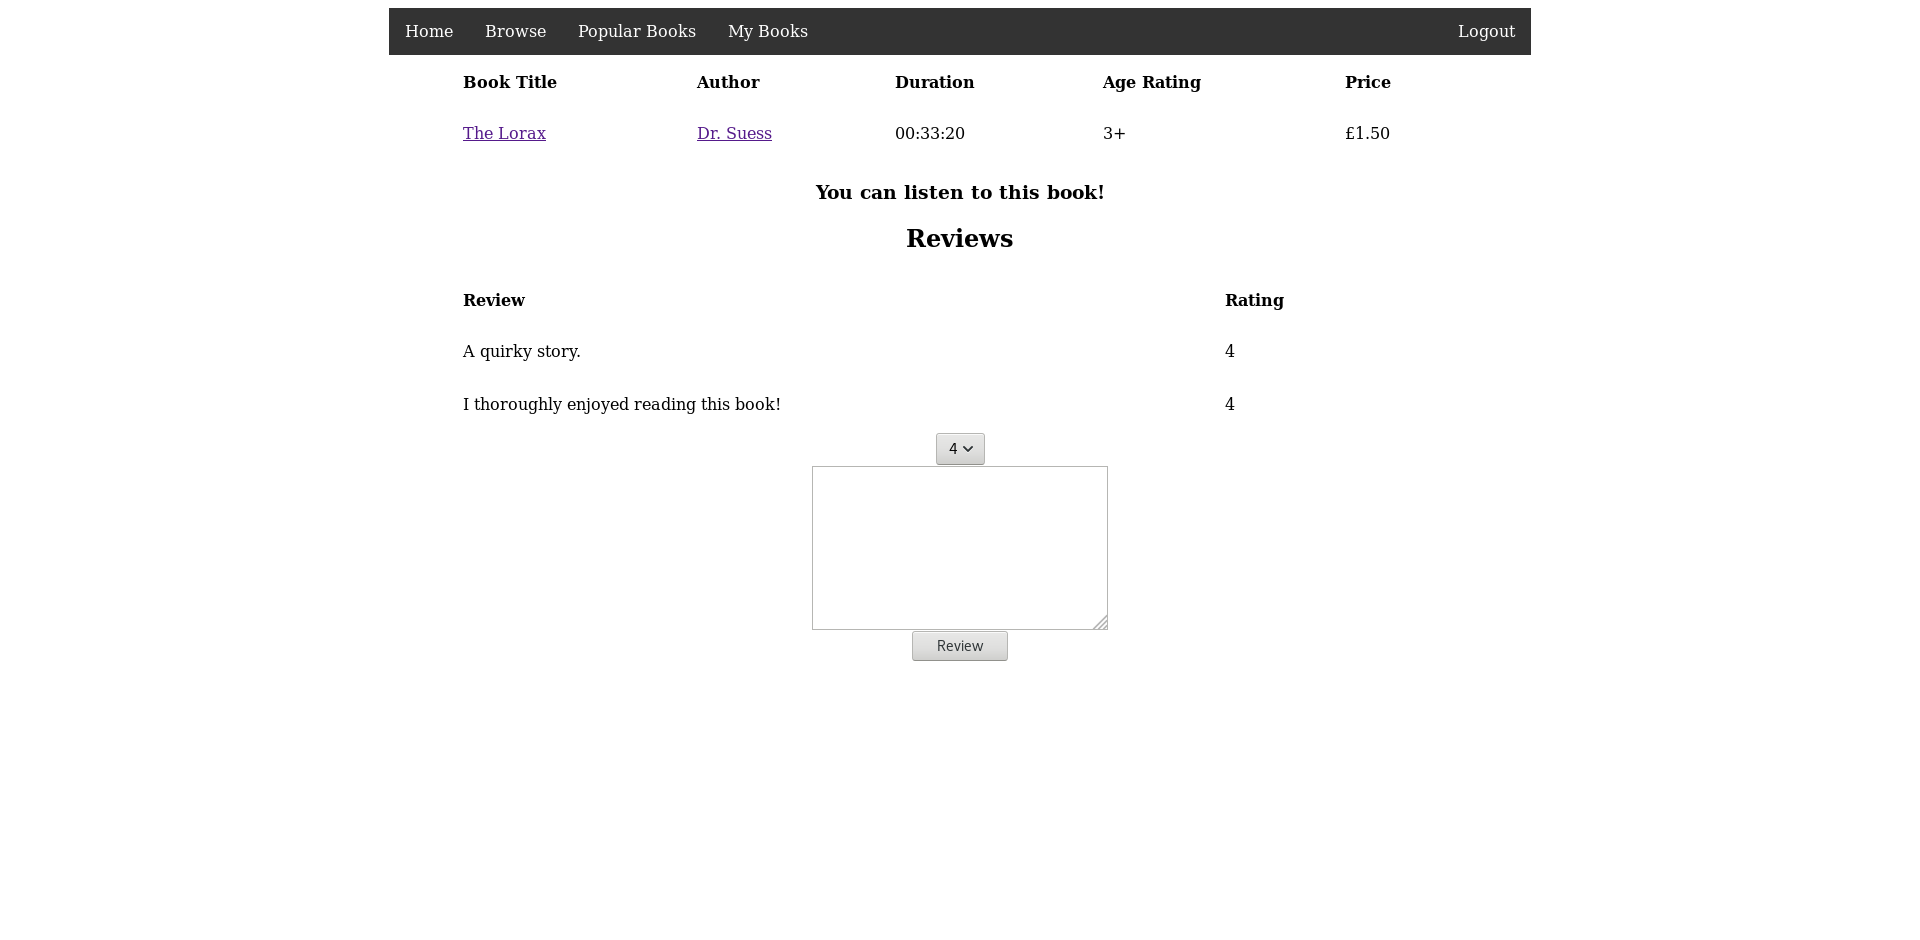
\includegraphics[scale=0.19]{image/book.png}
\end{figure}

\begin{figure}[!htb]
  \caption{An unpurchased book}
  \center
  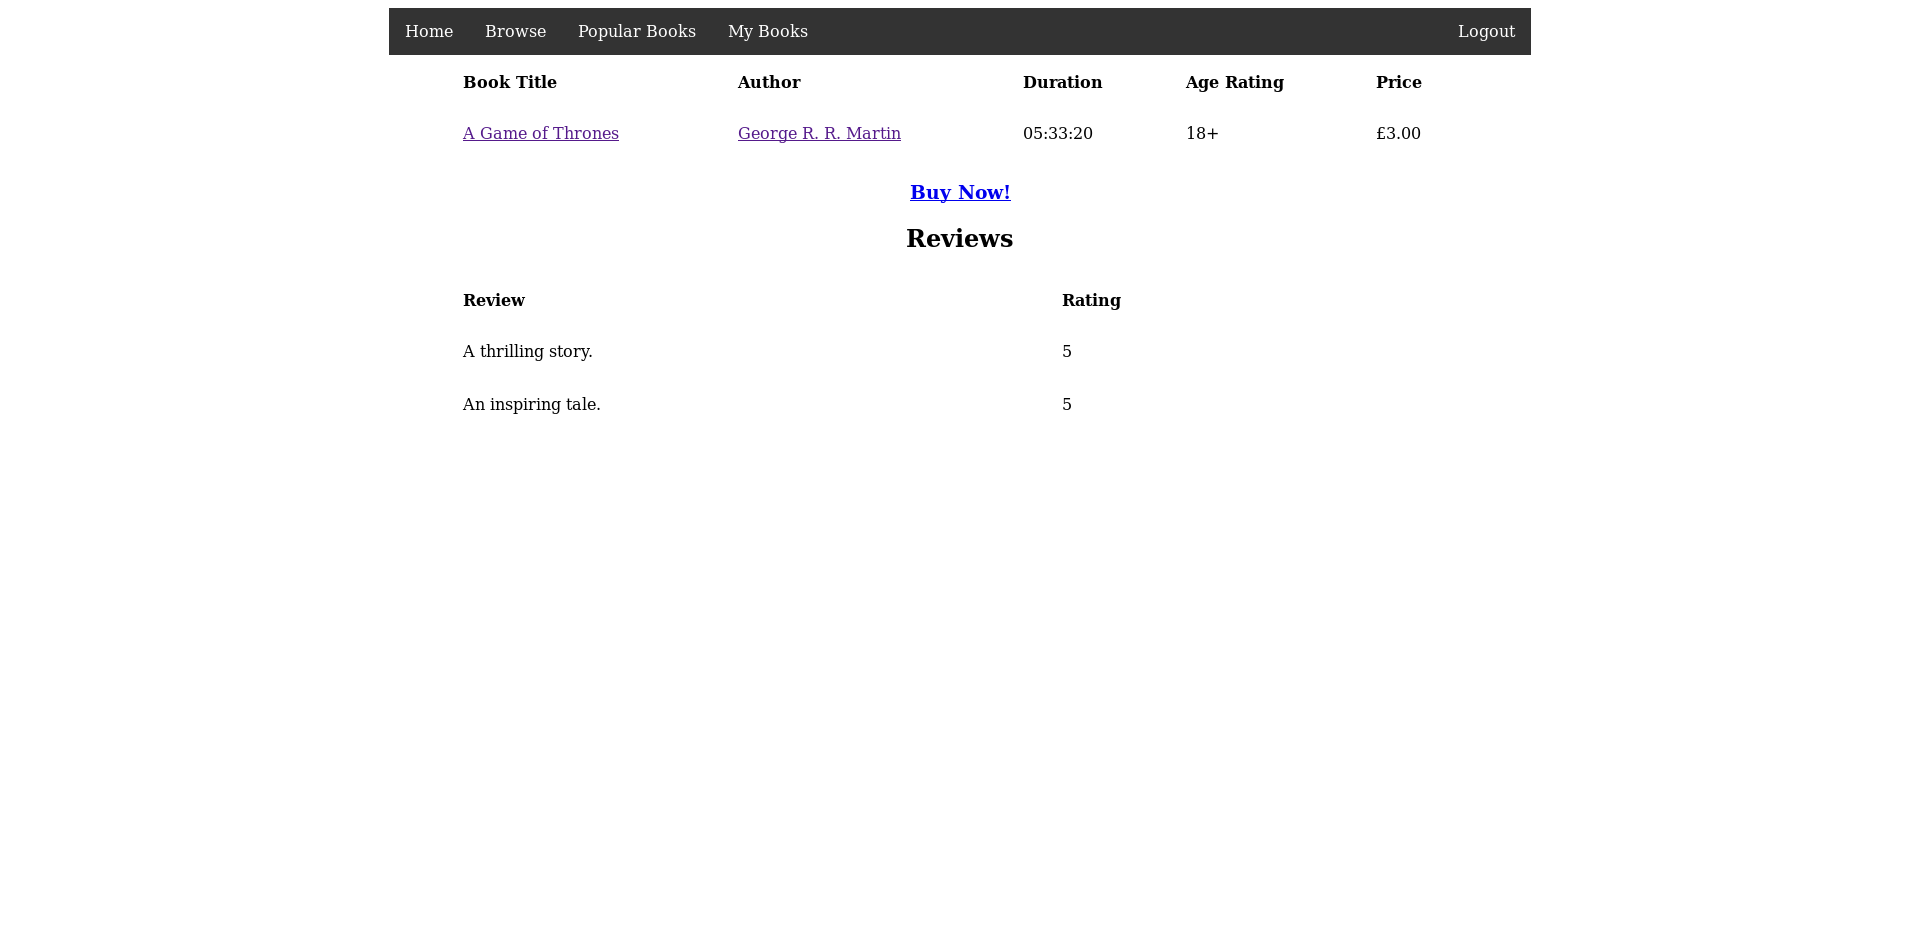
\includegraphics[scale=0.19]{image/book_b.png}
\end{figure}




\end{document}
